\documentclass[../exploring-pagerank.tex]{subfiles}

\begin{document}
	Deriving a limiting distribution from the Web graph, however, requires a bit more work. The real Web is quite reducible.
    \begin{figure}
        \centering
        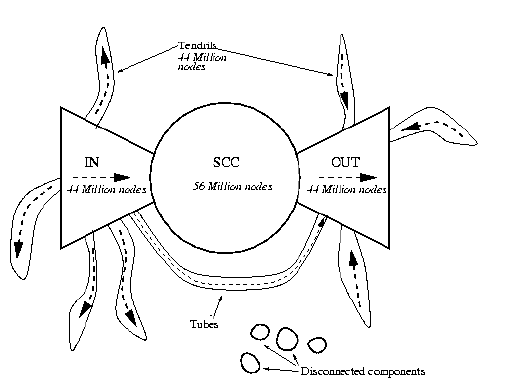
\includegraphics[scale=0.6]{bow-tie}
        \caption{The Bow Tie \cite{broderGraphStructureWeb}}
        \label{fig:bow-tie}
    \end{figure}
    In 1999, \cite{broderGraphStructureWeb} crawled over 1.5 billion links to generate a comprehensive map of the Web. Their macroscopic figure, given in Figure \ref{fig:bow-tie}, stylizes the Web super-graph as a rather eldritch bow tie. Note that the figure has the form of a directed acyclic graph given from a topological sort. In the middle is the ``bow knot'' -- the largest strongly-connected component (SCC) of the Web. In 2012, when the last public Web mapping occured, about half of mapped Web pages were strongly connected. The ``thistle ends'' of the tie, denoted \texttt{IN} and \texttt{OUT}, respectively reference pages from which surfers can link into (out of) the SCC but cannot return by the same route. Pages within the tendrils and tubes are likewise unidirectional on this macroscopic scale: They be reached from \texttt{IN} and \texttt{OUT}, but these components cannot be reached from within them. Although the numbers in \ref{fig:bow-tie} are obsolete, its bow-tie model wtill describes the Web well.

    We previously eliminated individual dangling pages, but we could view these entire tendrils and tubes again as ``dangling pages,'' and we can again correct for them. By our Markov discussion, we interpreted the stochastic Web matrix $S$ as the matrix of probabilities that an ideal random surfer follows links from a page or chooses another randomly when it hits a dead end. However, \textit{human} Web surfers often get bored. They will not follow a linear path through the Web; they might suddenly elect to teleport -- shift course altogether and visit a page on whim.
    Let $\mathbbm{1}$ represent a vector of ones, and again consider a distribution $u$ over all Web pages. We model this teleportation behavior with a rank-one matrix $T = \mathbbm{1}\transpose{u}$.

    Now, consider a matrix $G$ formed from a convex combination of $S$ and $T$:
	\begin{equation}
	    \label{eqn:google_matrix}
		G = \alpha S + (1-\alpha)T.
	\end{equation}
	Now, every page has some connection of nonzero probability to every other page, and our process is still stochastic. In fact, $G$ is trivially primitive, as each page has a random loop. In this model, the random surfer on page $p_i$ follows the Web's link structure about $\alpha s_i$ percent of the time and teleports with probability $(1-\alpha) u_j$. Note that the teleportation matrix need not give equal deference to each Web page. External factors -- a user's search preferences or browsing habits or a search engine's fiat against suspected abusers -- can influence the teleportation probabilities. Here, however, we take a rank-one distribution. The teleportation factor $\alpha$ dampens the wild, raw Web graph into a more friendly model; it is the damping factor.

	Note that the teleportation adjustment provides all we need for a guaranteed limiting distribution, from which we can directly rank pages. In sum, $G$ simply represents a lazy random walk on the Web graph $\mathcal{W}$. The matrix $G$ is the Google matrix -- the original foundation of PageRank calculations.

	Although the primitive Google matrix is completely dense, we can expand $S$ and $T$ into their constituent distributions $v$ and $u$ to obtain a power iteration:
    \begin{align*}
        \iterate{\pi}{k+1} &= \iterate{\pi}{k} G \\
        &= \alpha \iterate{\pi}{k} (H + d \transpose{v}) + (1 - \alpha) \iterate{\pi}{k} (\mathbbm{1} \transpose{u}).
    \end{align*}

    Note that the rank-one reduction given above does not require us to actually generate the dense component matrices $S$ and $G$. Unlike decompositional methods (e.g. UR factorization and GMRES), we do not ruin the sparsity of $H$. As we see above, we must only store the current iterate $\iterate{\pi}{k}$ and the dangling page vector $d$ to apply the power method. Our method does not require matrix multiplications, which have complexity $O(n^2)$. We need only perform vector-matrix multiplication on the very sparse $H$, and sparse multiplications have approximate complexity $O(\eta(H))$, where $\eta(H)$ is the number of nonzero elements in $H$. Empirical data shows the average Web page has about 10 outgoing links, so $\eta(H) \approx 10n$.

    Thus, when we apply the power method to a primitive matrix, we have an essentially linear algorithm. The power method beats more complex algorithms here because it gives only the simple result we want: the dominant eigenvalue of a primitive matrix. However, the convergence of a primitive Markov chain depends upon how quickly powers of its subdominant eigenvalue converge to zero. We now examine this eigenvalue more closely, and also investigate an optimum value for $\alpha$.
\end{document}
